%Results (chpt 07)
\chapter{Results} \label{chpt:results}
In this chapter we will evaluate the results of our final algorithm. To do so, we first create a test on which we can try out our algorithm, and measure its performance. We will begin by evaluating the mapping algorithm without the mapping strategy, by only initializing a map and testing it out. We will use this simple test to tune the parameters of bundle adjustment. Afterwards, we will evaluate the full mapping algorithm.\\

All experiments were carried out with the drone on a mobile platform. We did not work on the drone's controller or path planning, so to focus on the computer vision and mapping parts of the project we decided to move the drone manually instead of making it fly. 

\section{Evaluation procedure} \label{evalproc}
We will implement two tests to evaluate the quality of the map creation, the accuracy test, and the robustness test.\\

\subsubsection{Accuracy test}
During the accuracy test, the drone will first build a map, and then that map will be tested by comparing the real position of the drone with the one it estimates using the map and PnP. The setup used for this evaluation is illustrated on figure \ref{fig:benchmarksetup}.\\

The evaluation is performed as follows:
\begin{enumerate}
  \item The drone is placed in a predefined and known position on a table (position A in figure \ref{fig:benchmarksetup}). There, the drone is turned on, and it begins initializing its map by creating a first keyframe.
  \item The drone is then successively placed in 3 other known locations (B, then C, then D), and at each of these locations, the drone manually receives its position. Every time this happens, the drone creates a keyframe, adds landmarks into the map, and optionally updates existing landmarks' positions, or even removes some landmarks.
  \item Finally, the drone is again placed at different known locations (positions 1 through 4, then back to 1 on figure \ref{fig:benchmarksetup}). This time, no information is communicated to the drone from the outside, and the drone does not modify its map. The drone estimates its position using only its camera and the map that it built during step 2. While the drone is moved from point 4 to 1, its camera is obstructed, to test whether it can recover from being lost. At each point, we compare the drone's estimated position with its real position to evaluate the quality of the map.
\end{enumerate}
The two quantities we will seek to optimize are the accuracy of the drone's visual pose estimation (as measured during step 3), and the time taken to create the map during step 2.\\
\subsubsection{Robustness test}
In reality, the drone does not know its exact position when making keyframes at points B, C, and D (position A is defined as the origin). To emulate this, we implement a second type of test: the robustness test. The robustness test works exactly like the accuracy test, with as only difference that there is some error on the positions that are communicated to the drone at the points B, C and D. This serves to emulate the fact that the drone only has an estimate of its position when building the map and does not know it exactly.\\

We do not yet know what a realistic error would be on the position of the drone, so we will choose one arbitrarily, aiming to be pessimistic. At each of the three uncertain poses, we will do two of the following:
\begin{enumerate}
\item add \SI{30}{\centi\meter} to the $x$-coordinate.\\
\item add \SI{30}{\centi\meter} to the $y$-coordinate.\\ 
\item add \num{18}{\degree} to the yaw.\\
\end{enumerate}

\subsubsection{Performance measure}
For both the robustness and precision tests, we measure two quantities: the average distance error and average angle error. The average distance error is the average distance in the $xy$-plane between the drone's estimated position and its real position when it is at points 1, 2, 3, 4, then back at 1. The average angle error is the average absolute value of the difference between the estimated yaw angle and the real yaw angle at each of these positions. We do not take the errors on the altitude, as well as on the roll and pitch angles into account, because as explained in section \ref{sec:posefusion}, we do not use the result of the visual pose estimate for those quantities, but use the IMU and ultrasound directly. We also do not measure the error when we are moving the drone between the known positions, as we do not have equipment to measure its real position during those displacements.
\newpage
\begin{figure}[H]
  \centering
  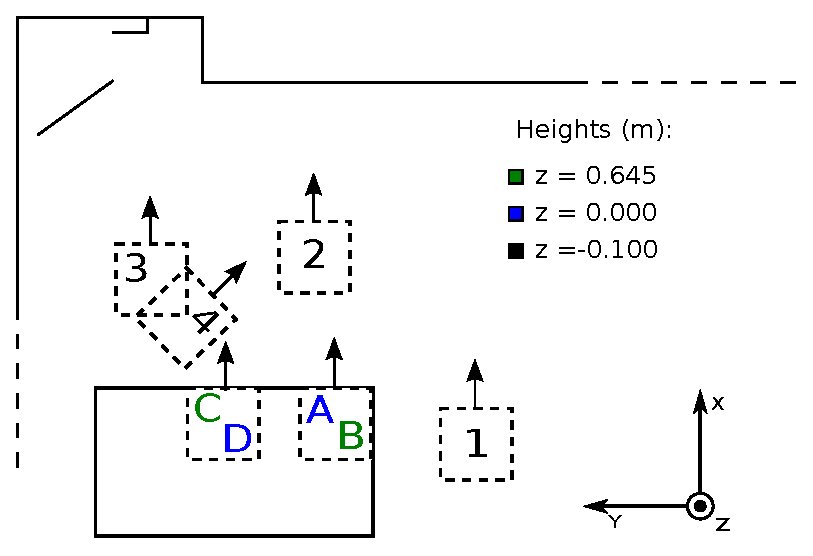
\includegraphics[width=\linewidth]{benchmark_setup_noground.eps}
  \caption{Different positions of the drone during the evaluation}
  \label{fig:benchmarksetup}
\end{figure}

\begin{figure}[H]
\centering
\begin{subfigure}{.24\textwidth}
  \centering
  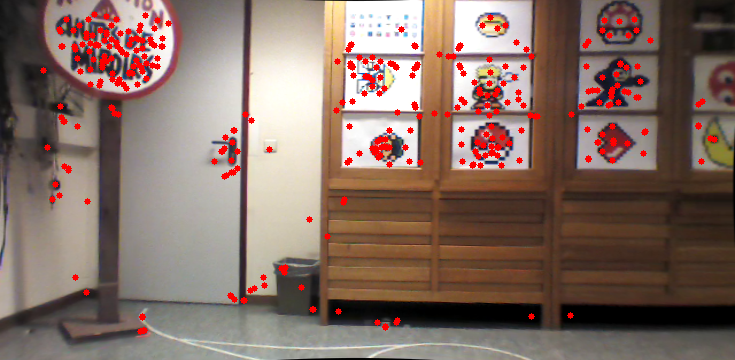
\includegraphics[width=.99\linewidth]{posA.png}
  \caption{View from position A}
  \label{fig:viewA}
\end{subfigure}
\begin{subfigure}{.24\textwidth}
  \centering
  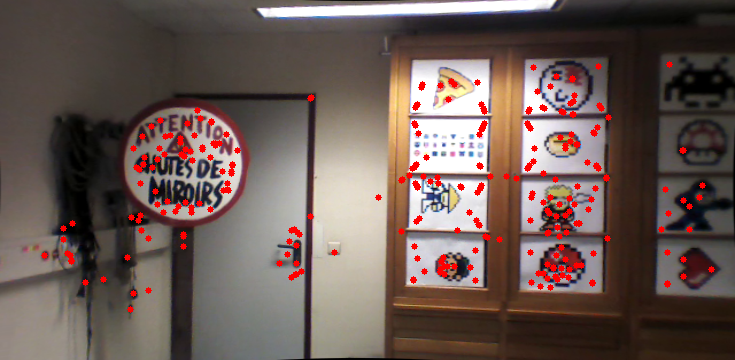
\includegraphics[width=.99\linewidth]{posB.png}
  \caption{View from position B}
  \label{fig:viewB}
\end{subfigure}
\begin{subfigure}{.24\textwidth}
  \centering
  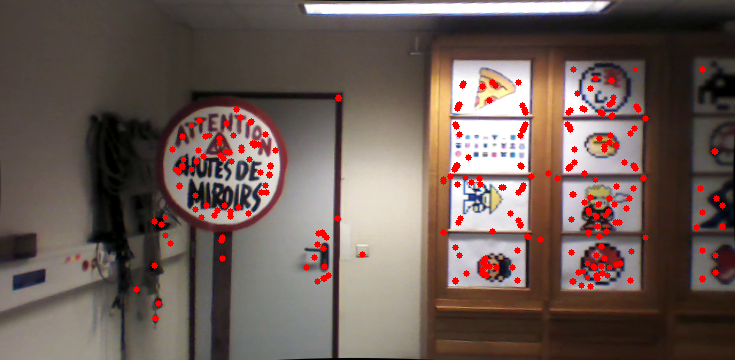
\includegraphics[width=.99\linewidth]{posC.png}
  \caption{View from position C}
  \label{fig:viewC}
\end{subfigure}
\begin{subfigure}{.24\textwidth}
  \centering
  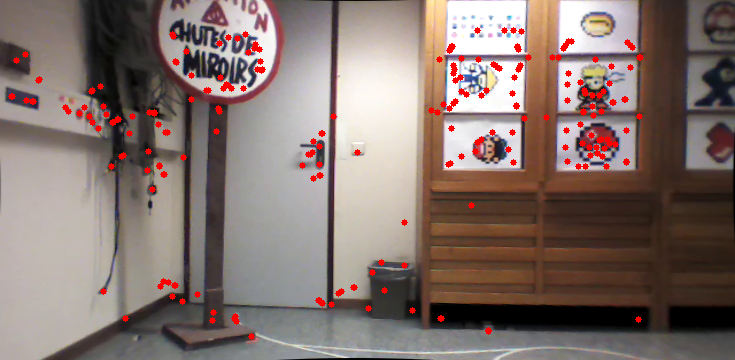
\includegraphics[width=.99\linewidth]{posD.png}
  \caption{View from position D}
  \label{fig:viewD}
\end{subfigure}\\

\begin{subfigure}{.24\textwidth}
  \centering
  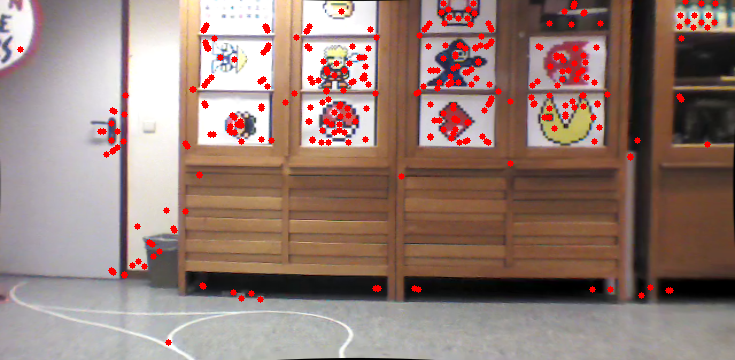
\includegraphics[width=.99\linewidth]{pos1.png}
  \caption{View from position 1}
  \label{fig:view1}
\end{subfigure}%
\begin{subfigure}{.24\textwidth}
  \centering
  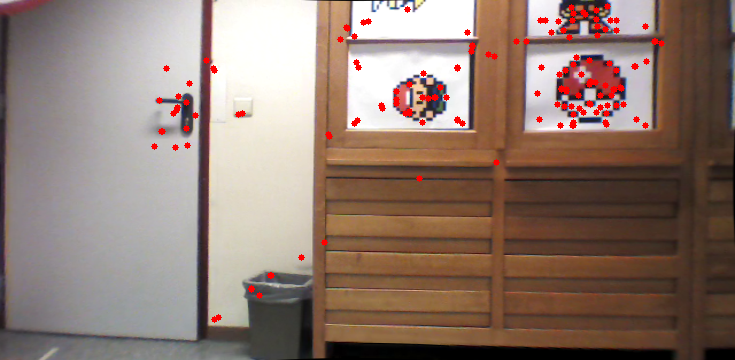
\includegraphics[width=.99\linewidth]{pos2.png}
  \caption{View from position 2}
  \label{fig:view2}
\end{subfigure}
\begin{subfigure}{.24\textwidth}
  \centering
  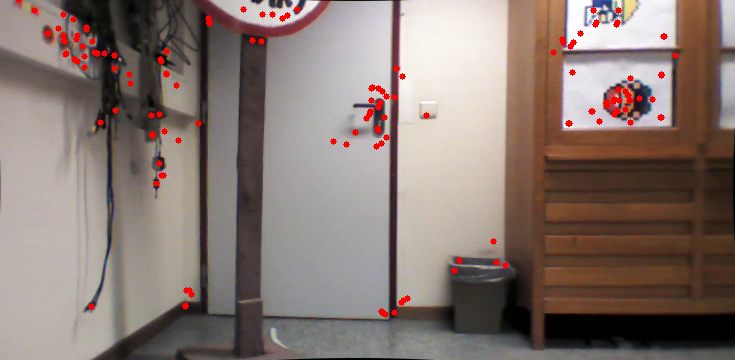
\includegraphics[width=.99\linewidth]{pos3.png}
  \caption{View from position 3}
  \label{fig:view3}
\end{subfigure}
\begin{subfigure}{.24\textwidth}
  \centering
  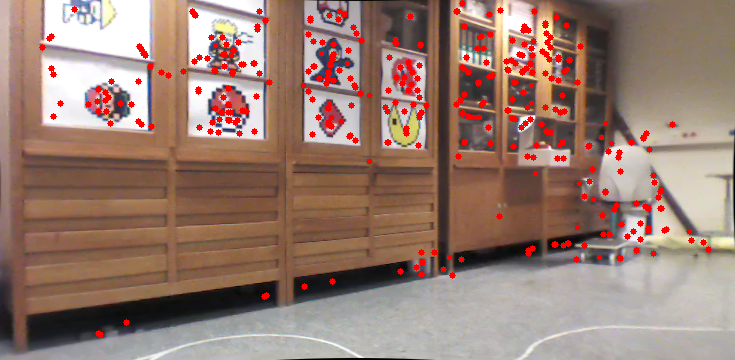
\includegraphics[width=.99\linewidth]{pos4.png}
  \caption{View from position 4}
  \label{fig:view4}
\end{subfigure}

\caption{Views during the evaluation}
\label{fig:benchmarkviews}
\end{figure}

\section{Comparison of triangulation methods} \label{sec:comparetriang}
Using the evaluation procedure described in section \ref{evalproc}, we can compare midpoint triangulation and optimal correction. A comparison of their performances on both tests can be seen on table \ref{fig:triangcompare}.

\begin{table}[H]
  \centering
  \caption{Comparison between triangulation methods}
  \small\addtolength{\tabcolsep}{-2pt}
  \sisetup{round-mode=places, round-precision = 3}
  \begin{tabular}{ @{} l S[table-format=2.2,round-precision=2] S[table-format=2.1,round-precision=1] @{\hspace{10mm}}
                         S[table-format=2.2,round-precision=2] S[table-format=2.1,round-precision=1] @{}  }
    \toprule
    {}                 & \multicolumn{2}{c}{Accuracy test} &  \multicolumn{2}{c}{Robustness test} \\
    {}                 & {\footnotesize Distance (\si{\meter})} & {\footnotesize Angle}
                       & {\footnotesize Distance (\si{\meter})} & {\footnotesize Angle} \\
    \midrule
    Midpoint Method    & \num{0.121729436669}  & \SI{2.9988106732981}{\degree} & \num{0.844616151792} & \SI{15.48115281064}{\degree}\\
    Optimal Correction & \num{0.0988557438948} & \SI{2.3287093550318}{\degree} & \num{0.775954169079} & \SI{12.52132481967}{\degree}\\
      \bottomrule
  \end{tabular}
  \label{fig:triangcompare}
\end{table}

We can see that the optimal correction method performs somewhat better. However, this comes at the cost of computation time, because it takes approximately \SI{12}{\milli\second} to triangulate all \num{165} matches between two views using the midpoint method, and \SI{24}{\milli\second} to do the same with the optimal correction method. In both cases however, this time is insignificant when compared to bundle adjustment (which is performed just after triangulation). For this reason, and the fact that optimal correction is better motivated theoretically and that it gives slightly better results, we will use optimal correction.\\

It is interesting to see, however, that the difference in performance is much greater between the accuracy and robustness tests than between the two triangulation methods. This can be explained by the fact that optimal correction is well suited to correct measurement errors that follow a normal distribution, but not errors stemming from the fact that the position estimate of the cameras is inexact. That is the reason why we need bundle adjustment.

\section{Bundle Adjustment}
\begin{table}[H]
  \centering
  \caption{Performance of Bundle Adjustment}
  \small\addtolength{\tabcolsep}{-2pt}
  \sisetup{round-mode=places, round-precision = 3}
  \begin{tabular}{ @{} l S[table-format=2.2,round-precision=2] S[table-format=2.1,round-precision=1] S[table-format=2.3,round-precision=3]
                         S[table-format=2.2,round-precision=2] S[table-format=2.1,round-precision=1] S[table-format=2.3,round-precision=3] @{}  }

    \toprule
    {}      & \multicolumn{3}{c}{Accuracy test } &  \multicolumn{3}{c}{Robustness test} \\
    {}      & {\scriptsize Distance (\si{\meter})} & {\scriptsize Angle} & {\scriptsize Time (\si{\second})}
            & {\scriptsize Distance (\si{\meter})} & {\scriptsize Angle} & {\scriptsize Time (\si{\second})} \\
    \midrule
    No B.A.  &\num{0.0988557438948}&\SI{2.3287093550318}{\degree}&{\textemdash}&\num{0.775954169079}&\SI{12.52132481967}{\degree}&{\textemdash}\\
    With B.A.&\num{0.0776431}      &\SI{1.25765337}{\degree}     &\num{0.775227}
             &\num{0.16953509}     &\SI{3.76480354}{\degree}     &\num{1.835684}  \\
    \bottomrule
  \end{tabular}
  \label{tab:bacompare}
\end{table}

We can see on table \ref{tab:bacompare} that bundle adjustment improves the results of both the accuracy and the robustness tests. The improvement is significant in the accuracy test, but it is especially large in the robustness test. This first little experiment convinces us that bundle adjustment really works, and is a good way to correct errors coming from imprecise pose estimation. The improvement of the performance in the accuracy test can be explained by the fact that even if we tried giving the drone its exact position when it was building the map, the information we sent was not \SI{100}{\percent} exact, and these inaccuracies were corrected by bundle adjustment.\\

The performance increase gained from bundle adjustment comes at a price in the form of computation time. Table \ref{tab:bacompare} shows that bundle adjustment took a total of \SI{0.775}{\second} during the accuracy test, and \SI{1.836}{\second} during the robustness test. This time is the total time for all three rounds of bundle adjustment run during the initialization phase (it runs every time a keyframe is created, except for the first keyframe). As we can see on table \ref{tab:batime}, the time taken by the algorithm increases each time it is ran, because the map grows. Because bundle adjustment is ran every time a keyframe is created but not at every new image, relatively large times are acceptable. However, long times for bundle adjustment limit the speed at which the drone can explore, so we want to keep it under control. We will explore some ideas to keep this computation time low, while still having a good enough performance. \\
\newpage
\begin{table}[H]
  \centering
  \small\addtolength{\tabcolsep}{-2pt}
  \sisetup{round-mode=places, round-precision = 3}
  \begin{tabular}{ @{} l @{\hspace{10mm}}
      S[table-format=3.0] S[table-format=1.2,round-precision=2] S[table-format=1.3,round-precision=3] @{\hspace{10mm}}
      S[table-format=3.0] S[table-format=1.2,round-precision=2] S[table-format=1.3,round-precision=3] @{}  }
    \toprule
    {} & \multicolumn{3}{l}{Accuracy Test} & \multicolumn{3}{l}{Robustness Test} \\
    {} & {$N$} & {$\alpha$} & {Time [\si{\second}]} & {$N$} & {$\alpha$} & {Time [\si{\second}]} \\
    \midrule
    Bundle Adjustment 1 & \num{112} & \num{2}        & \num{0.085864} & \num{112} & \num{2}        & \num{0.213027} \\
    Bundle Adjustment 2 & \num{277} & \num{2.404332} & \num{0.369665} & \num{277} & \num{2.404332} & \num{0.636927} \\
    Bundle Adjustment 3 & \num{340} & \num{2.561765} & \num{0.319698} & \num{339} & \num{2.560472} & \num{0.985730} \\
    \midrule
    \textbf{Total}      & {} & {} & \num{0.775227} & {} & {} & \num{1.835684} \\
    \bottomrule
  \end{tabular}
  \caption{Bundle adjustment timings during the initialization step of a benchmark test. $N$ is the number of points being adjusted, $\alpha$ is the average number of times each point is observed.}
  \label{tab:batime}
\end{table}

We already notice the difference in the time it takes for the robustness and accuracy tests. Bundle adjustment is an iterative algorithm that seeks to minimize a certain cost function. Because during the accuracy test we start from closer to the solution, it requires fewer iterations to correct the errors, so the better our position estimates, the faster bundle adjustment will run. This explains why bundle adjustment is takes more time for the robustness test than for the accuracy test


\subsection{Tuning the Bundle Adjustment}
There are many different parameters for bundle adjustment that can be tuned. We will try to find the best balance between performance and speed. Because there is a high variance on the performance on the tests, we will carry out each test multiple times to give an estimate of the performance of each set of parameters, and compare both the average performance, and the worst-case performance of the different sets of parameters. During this tuning phase, we will only perform the robustness test, as the performance on the accuracy test is already quite good, and does not vary much between the tests.

\subsubsection{Outlier threshold}\label{sec:outliers}
After each round of bundle adjustment, we consider points to be outliers if their reprojection error is above some threshold. If an outlier is seen by only two keyframes, it is removed from the map. If it is seen by more, then we only disregard the last observation of this landmark, because if it was still present in the map, that must mean that it wasn't an outlier before that last observation was taken into account. The loss function we are using (Huber's loss) is already designed so that outliers' contribution to the objective function is not too high, so it makes sense to tune its parameter $\delta$ at the same time as the threshold for removing points considered outliers.\\

\subsubsection{Convergence of the solver}
We can also tune the convergence criterion of the solver that solves the bundle adjustment problem. We will stop when the ratio of the change in the objective function to the value of this function arrives below some threshold. This ensures that the criterion scales with the problem, which is important as the size of the problem can vary during operation (as the map grows, for example). The default value of the Ceres solver is $10^{-6}$, but experimentally, we find that this gives very bad results, and takes quite a long time.\\

After this tuning, we are able to bring the average error during the robustness test down to the following values:
\begin{table}[H]
  \centering
  \caption{Performance after tuning the bundle adjustment}
  \small\addtolength{\tabcolsep}{-2pt}
  \sisetup{round-mode=places, round-precision = 3}
  \begin{tabular}{ @{} l S[table-format=2.2,round-precision=2] S[table-format=2.1,round-precision=1] S[table-format=2.3,round-precision=3] @{}  }

    \toprule
    {}      & {\scriptsize Distance (\si{\meter})} & {\scriptsize Angle} & {\scriptsize Time (\si{\second})} \\
    \midrule
    Before tuning  &\num{0.16953509}     &\SI{3.76480354}{\degree}     &\num{1.835684}  \\
    After tuning   &\num{0.114956201}    &\SI{1.999336913}{\degree}    &\num{1.8251724496}\\
    \bottomrule
  \end{tabular}
  \label{tab:batuning}
\end{table}

\subsection{Final results of bundle adjustment}

\begin{figure}[H] %fig:ptcloud
\centering
\begin{subfigure}{0.49\textwidth}
	\centering
  	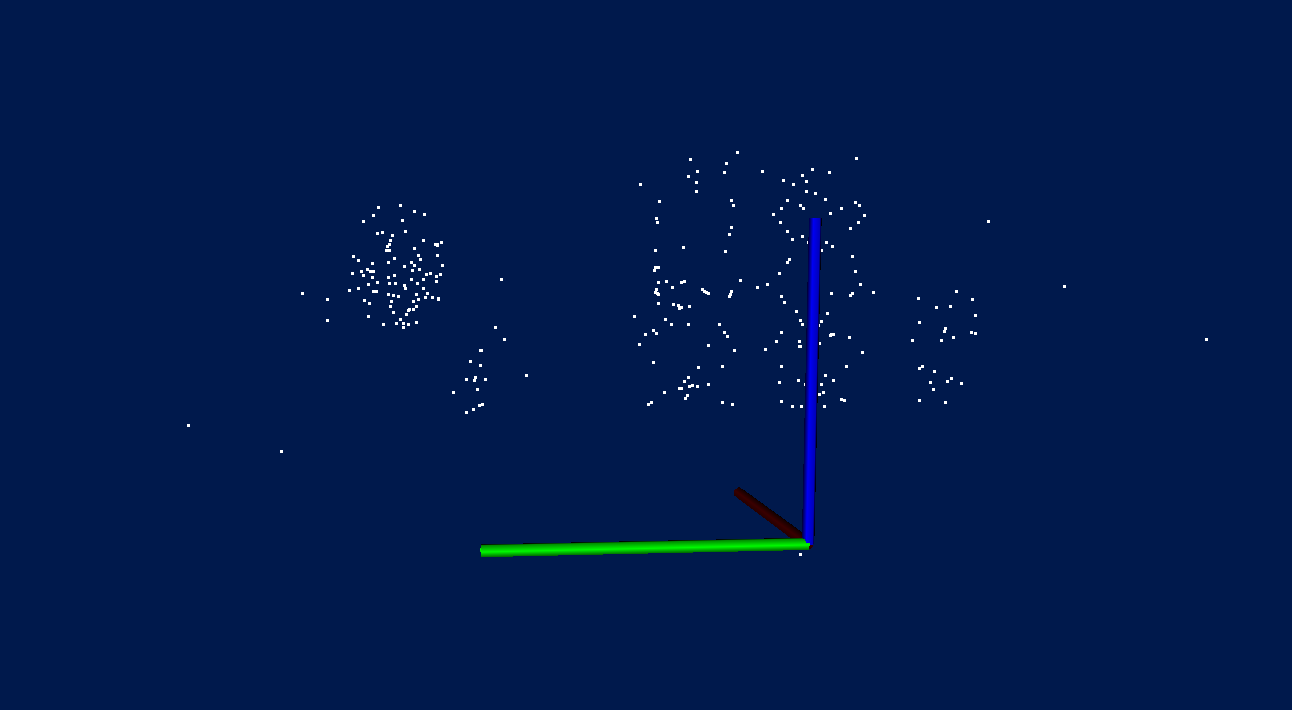
\includegraphics[width=\linewidth]{vanillaBA_robust_front.png}
	\caption{Front view, with bundle adjustment}
	\label{fig:ptcloud_ba}
\end{subfigure}
\begin{subfigure}{0.49\textwidth}
    \centering
	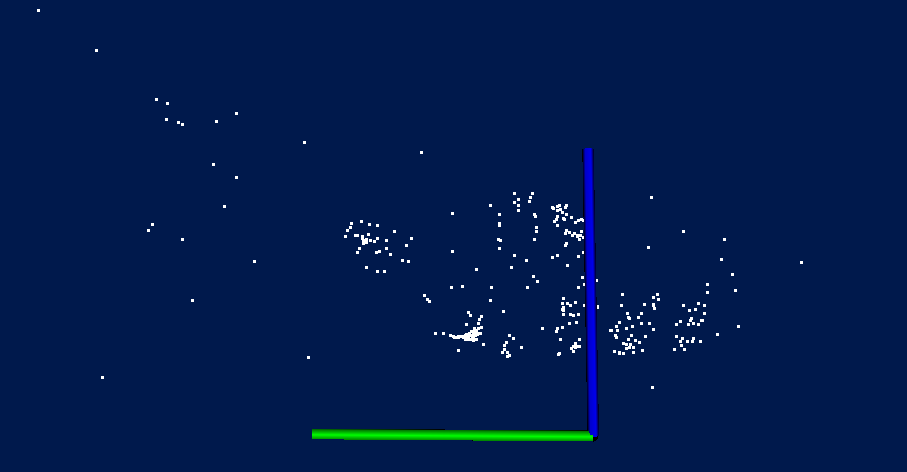
\includegraphics[width=\linewidth]{noBA_robust_front.png}
	\caption{Front view, no bundle adjustment}
	\label{fig:ptcloud_noba}
\end{subfigure}\\

\begin{subfigure}{.49\textwidth}
  \centering
  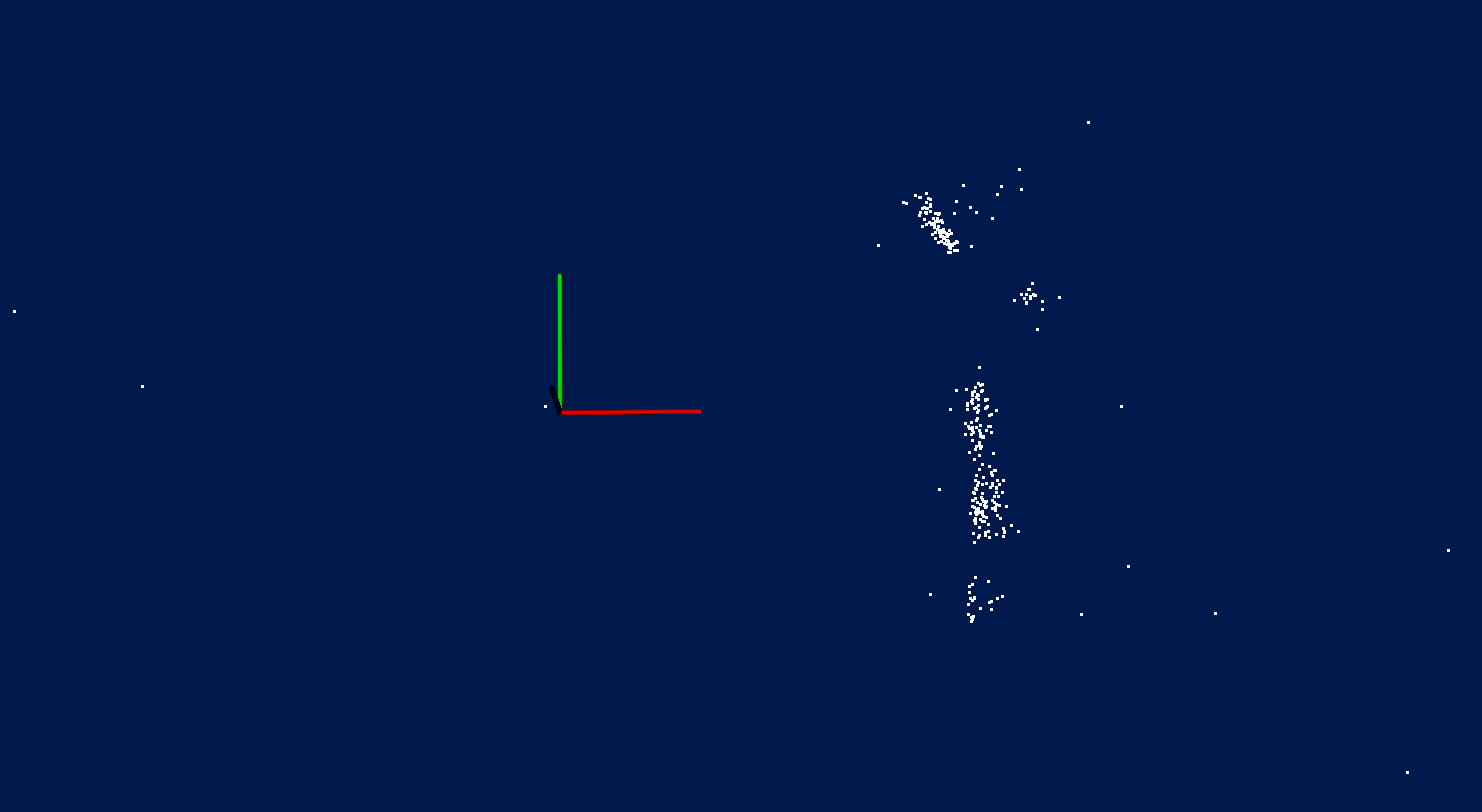
\includegraphics[width=\linewidth]{vanillaBA_robust_zoom.png}
  \caption{Top View, with bundle adjustment}
  \label{fig:ptcloud_vanillaBA_robust}
\end{subfigure}
\begin{subfigure}{.49\textwidth}
  \centering
  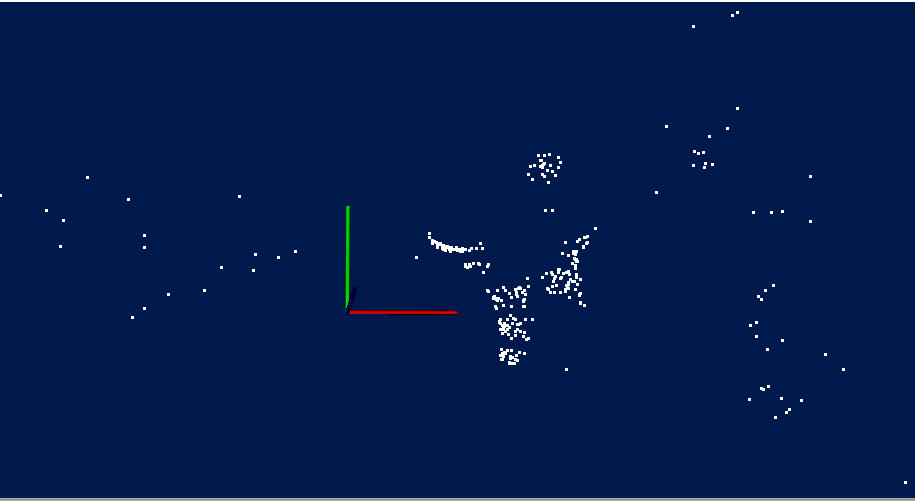
\includegraphics[width=\linewidth]{noBA_robust_zoom.png}
  \caption{Top view, no bundle adjustment}
  \label{fig:ptcloud_noBA_robust}
\end{subfigure}%

\caption{Point clouds after initialization during the robustness test}
\label{fig:ptcloud}
\end{figure}

Figure \ref{fig:ptcloud} shows the map created by the drone during the robustness test, with and without bundle adjustment. With bundle adjustment, we can recognize the sign, the cabinet, and the door handle from figure \ref{fig:benchmarkviews}, and from the top view we can see that these structures are quite planar. Without bundle adjustment, however, the map is unrecognizable.\\

Figure \ref{fig:xyyaw_traj} compares the estimated trajectory of the drone during the robustness test, with the real reference positions. We can see that the largest error made is about \SI{20}{\centi\meter} of distance in the $xy$-plane and \SI{5}{\degree} of yaw-error. For the applications we are considering, these errors are at the limit of what is acceptable, because the drone we are using is \SI{51}{\centi\meter} wide with its indoor hull, and it could just not pass a door (\SI{90}{\centi\meter} wide) with \SI{20}{\centi\meter} on either side. \\

Despite being on the limit in the worst case, we are satisfied with this result, because the robustness test only tests the general useability of bundle adjustment and not of the entire mapping algorithm, as no new keyframes are created after the initialization. On Figure \ref{fig:xyyaw_traj}, we see that the largest errors were made at position 3, more than \SI{80}{\centi\meter} away from the closest keyframe, and more than \SI{80}{\second} later. We can also see on figure \ref{fig:view3} that the overlap between its field of view and the ones at positions A, B, C and D is quite small. During real operation, the drone would have created more keyframes during its displacement towards position 3, so when arriving there, it would have more landmarks in its field of view. For this reason, we believe that the errors made at positions 1, 2, and 4 are more indicative of the real performance of our map.\\

The straight lines between positions 4 and 1 correspond to the time during which the camera of the drone is blocked. During this time, the drone does not publish a visual estimation of its position. We can see that after this occlusion, the drone is capable of finding its position again.

\begin{figure}[H]
  \centering
  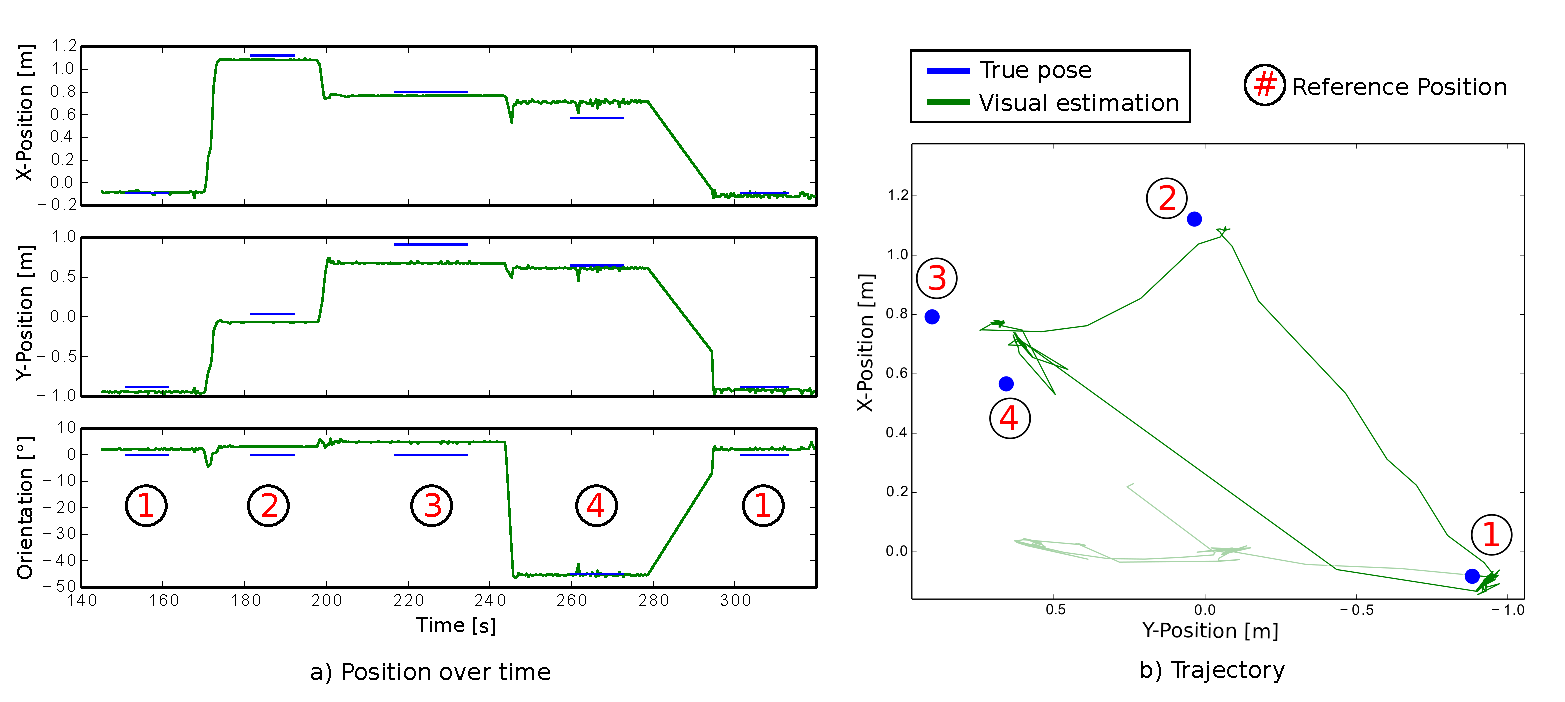
\includegraphics[width=\linewidth]{allresult_barobust.eps}
\caption{Result of robustness test with bundle adjustment. The four positions correspond to the ones of the evaluation, as shown on figure \ref{fig:benchmarksetup}. The grayed-out part of the trajectory corresponds to the initialization of the map (positions A through D)}.
\label{fig:xyyaw_traj}
\end{figure}

\section{Mapping strategy}
Now that we tested how well bundle adjustment works to create a map, and that we convinced ourselves that it is capable of recreating the 3D geometry of the world, we need to test the mapping algorithm itself (which was explained in section \ref{sec:heuristic}). Unfortunately, the limited access to the sensors when the drone isn't flying means that it is very difficult to recreate realistic conditions regarding the information the drone has. Regardless, for simple trajectories, such as pure translations, the algorithm works quite well. Unfortunately, for longer trajectories, the scale problem ends up making the tests fail.

\subsection{Difficulties for testing the mapping strategy}\label{sec:difficult}
It is much more difficult to test our mapping strategy than is was to test the mapping itself, because we do not know in advance when the drone will create keyframes. This poses a problem, because our drone isn't flying during the tests, so we don't have access to the ultrasound. As a result, we have to either manually communicate its altitude to the drone during the entire flight, or use the drone's height estimation from PnP as if it were the ultrasound's estimation. Both approaches have disadvantages.\\

If we communicate its altitude manually to the drone, that means the drone has to stay at the same altitude during the entire test, because we would not be able to give it its exact altitude during transitions from one to another. If the drone stays at the same altitude throughout the test, the soft constraint we put on the keyframes' altitudes don't fix the scale anymore, because they do not put any constraint on the distance between keyframes. In that case, the only thing fixing the scale are the two keyframes that are held constant during local bundle adjustment, but they are also subject to drift.\\

If we use the drone's visual estimation of the altitude as if it were the ultrasound sensor, the scale also drifts, because the visual estimation depends on the map, so errors accumulate.\\


\subsection{Short trajectories}
Despite the problems explained in section \ref{sec:difficult}, the heuristic developed in section \ref{sec:heuristic} works quite well when the drone carries out short trajectories. On figure \ref{fig:heuristic}, we can see the resulting map from the drone moving in a straight line to the right after initialization. During initialization, only the part to the left of the black line was visible by the drone, and as it moved away, it created keyframes, and proceeded with local and global bundle adjustment as explained in section \ref{sec:mapstrat}. At the end of its trajectory, none of its field of view contained parts of the initial map. We see that it worked, well, because the scene seems planar on the map, as it is in real life. However, there are still many points that seem to be outliers that weren't removed.\\

\begin{figure}[H]
  \centering
  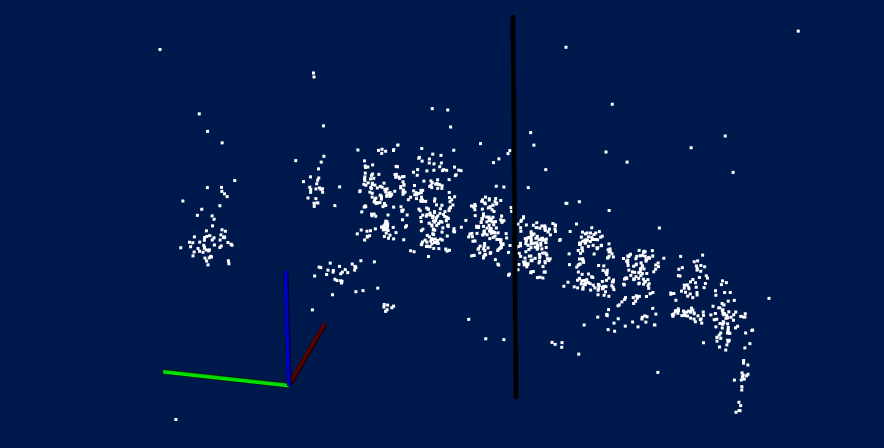
\includegraphics[width=0.5\linewidth]{heuristic_straightline_separated.png}
\caption{Map resulting from free exploration}
\label{fig:heuristic}
\end{figure}

\subsection{Long trajectories}
For longer trajectories, the performance quickly deteriorates. We are convinced that the reasons explained in section \ref{sec:difficult} are to blame for this deterioration. Unfortunately, with the available equipment, we were not able to devise a test that realistically gave the drone an altitude measurement that corresponds to one measured by the ultrasonic sensor, while also varying this altitude during the test. We are certain that the results would be much better on such a test.\\

We attempted to make the drone carry out a full loop, to be able to run global bundle adjustment at the end of the loop, correcting any accumulated errors. Unfortunately, as we moved away from the initial keyframes, the accuracy of the map became poorer, until it could no longer be used by the drone.

\subsection{Loop closure}
The attempt to carry out a full loop to test out the mapping strategy failed, but we would still like to see  if our algorithm is able to successfully carry out loop closure.\\

To show that loop closure does work, we finally carried out a test without the mapping strategy, where we manually told the drone when to create keyframes during the entire experiment. This allowed to resolve the problems cited in section \ref{sec:difficult}, because as we tell the drone when to create a keyframe, we can also give it its exact altitude, even if this altitude is not constant. By working this way, we were able to carry out a full loop, mapping an entire room in the process. The resulting final map can be seen on figure \ref{fig:fulloop}.\\

\begin{figure}[H]
  \centering
  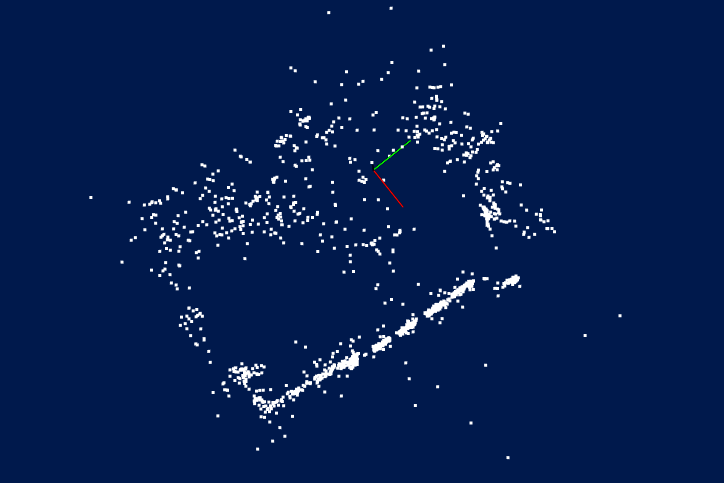
\includegraphics[width=0.5\linewidth]{fulloop.png}
\caption{Map resulting from a full loop, where keyframes were added manually (top view)}
\label{fig:fulloop}
\end{figure}
